\documentclass[margin,line,a4paper]{resume}
 
\usepackage{polyglossia}
\setdefaultlanguage{danish}
\usepackage[none]{hyphenat}
\usepackage{graphicx,wrapfig}
\usepackage{url}
\usepackage{fontspec}
\usepackage{xltxtra}
\setmainfont{Minion Pro}
\usepackage[colorlinks=true, a4paper=true, pdfstartview=FitV,
linkcolor=blue, citecolor=blue, urlcolor=blue]{hyperref}
\frenchspacing
 
\begin{document}
\raggedright
{\sc \Large Curriculum Vitae -- Martin Bjeldbak Madsen}
\begin{resume}
    \vspace{0.5cm}
    \begin{wrapfigure}{R}{0.6\textwidth}
         \vspace{-1cm}
        \begin{center}
        \reflectbox{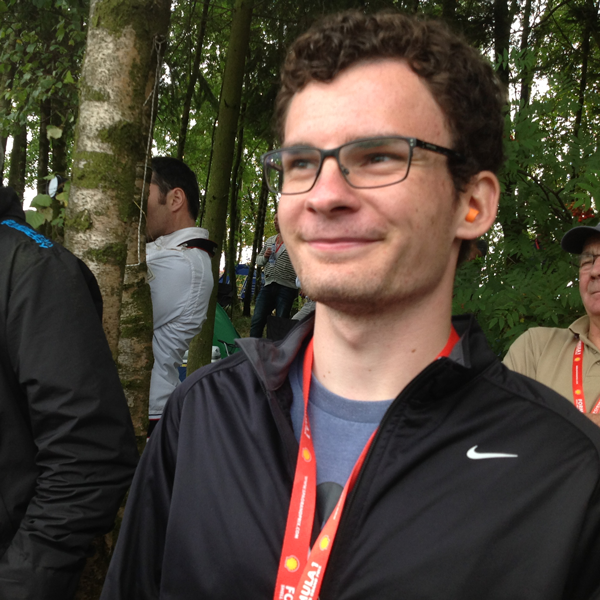
\includegraphics[width=0.6\textwidth]{moi.png}}
        \end{center}
         \vspace{-2cm}
    \end{wrapfigure}

    \section{\mysidestyle Personlig\\Information}%\vspace{2mm}
    Martin B.\ Madsen\\
    9.\ juni 1992 (21 år)\\ 
    Langagervej 4, st 108\\
    9220 Aalborg Øst\\
    Danmark\\
    Mobil: 26 27 36 60\\
    \href{mailto:martin2madsen@gmail.com}{martin2madsen@gmail.com}\\
    \href{http://www.martinbmadsen.dk}{martinbmadsen.dk}\\
    \href{http://dk.linkedin.com/pub/martin-madsen/21/9b0/b0}{LinkedIn - Martin Madsen}\vspace{1cm}

    Født og opvokset i Danmark til jeg var 5 år, hvorefter vi havde et
    9-år langt ophold i udlandet både i England og USA. Så jeg er vant
    til at tale engelsk og dansk med de lokale, samt tilpasse mig til
    nye miljøer. Jeg bor selvstændigt og vil gerne arbejde inden for
    computere eller med mennesker i it-branchen som et supplement til
    mit studie.

    I øjeblikket studerer jeg datalogi på Aalborg Universitet. Her går
    jeg på 5.\ semester og engagerer mig i nogle spændende projekter
    baseret på en dynamisk grundlag bygget op på problembaseret
    gruppearbejde! Vi har f.\ ek.\ designet op implementeret et
    programmeringssprog fra bunden af, der skal gøre det lettere, at
    hurtigt kunne skrive brætspil for derefter at spille dem direkte,
    enten mod computeren eller en anden spiller. Dette semester
    indeholder kurser om maskinintelligens, hvilket jeg virkelig glæder
    mig til!

    Jeg har har haft dansk kørekort til bil i 3 år.

    \section{\mysidestyle Uddannelse}
    Jeg har hvad der ligner en meget almen uddannelsesbaggrund. I
    fremtiden skal jeg til udlandet (USA) på det første år af min
    kandidat, hvorefter den færdiggøres på Aalborg Universitet.

    \textbf{Aalborg Universitet - Bachelor i Datalogi}
      (2011 - 2014) Jeg afslutter 6.\ semester, min bachelor, juni
      2014. Kandidaten afleveres i løbet af sommeren 2016.

    \textbf{EUC Nord - HTX} (2008 - 2011) Teknisk gymnasium i Hjørring.
      Naturvidenskabelig linje (Matematik A, Fysik A) samt Dansk A med
      Engelsk A som valgfag.

    \textbf{Bagterpskolen} (2006 - 2008) Folkeskole i Hjørring.

    \textbf{J. R. Gerrits Middle School} (2003 - 2006) Elementary og
      Middle School i Kimberly, Wisconsin, USA.

\section{\mysidestyle Professionel\\erfaring}\vspace{1mm}
\begin{description}

  \item[2012 sept $\rightarrow$ nu] Studenterprogrammør hos Falck
    Healthcare a/s. Hovedsaglig webudvikling i Ruby on Rails på et internt
    system.

  \item[2010 sept $\rightarrow$ nu] Startede enkeltmandsvirksomheden
    \emph{Divambu}. Virksomheden har fokus på udvikling og hosting af
    hjemmesider samt konsultentservicer inden for IT og computere. På
    \url{divambu.dk} ses en portfolio af projekter jeg har gennemført for
    kunder. Hobbyvirksomhed med lav omsætning.

  \item[2009 feb $\rightarrow$ 2010 jun] Ungarbejder ved Fakta
    a/s. Jobfunktionerne bestod i at side ved kassen, fylde varer op,
    ordne dagligdags butiksarbejde, osv. Meget af jobbet bestod af at have
    kontakt med kunderne, forstå deres problem, og derefter løse det.
\end{description}

\section{\mysidestyle Andet aktivitet}\vspace{1mm}
\begin{description}
  \item[2012 juli $\rightarrow$ nu] Mentor, Projekt
    \href{http://www.urk.dk/solskinsunge/}{Solskinsunge} 2012. Frivillig
    arbejde, hvor vi arrangerer sociale arrangementer med socialt udsatte
    børn fra Tornhøjskolen i Aalborg Øst.

  \item[2012 sept $\rightarrow$ august 2013] Hej \\ 
    \includegraphics[scale=0.05]{unf-logo.jpg}
    Sponsoransvarlig, UNF
    \href{http://software.unf.dk}{Software Development Camp} der
    fandt sted i sommeren 2013. Frivillig arbejde for Ungdommens
    Naturvidenskabelig Forening (UNF), hvor jeg opretter og holder
    kontakten med de forskellige sponsorer, der sørger for, at campen kan
    holdes.
\end{description}

\section{\mysidestyle Kompetencer} \vspace{1mm}
Jeg kan hurtigt sætte mig
ind i noget nyt, men der er nogle særlige emner, der især interesserer
mig:
\vspace{0.5cm}
\begin{description}

  \item[Styresystemer] Grundlæggende forståelse for de fleste
    Unix-lignende systemer: Ubuntu, Debian, CentOS, Arch Linux og Mac OS
    X.

  \item[Servere og databaser] Nginx. 

  \item[CMS-systemer] Jeg har opsat systemer med Wordpress, phpBB,
    Octopress.

  \item[Versionskontrolsystemer] Git, SVN.

  \item[Programmering-, scripting- og markupssprog] \LaTeX{} og
  \XeTeX{}, HTML, CSS, C, C\#, Java, JavaScript og jQuery, Ruby og Ruby
  on Rails.

\end{description}

\section{\mysidestyle Sproglige kompetencer}
Mit modersmål er dansk, men næsten alt det jeg laver er på engelsk,
både i forbindelse med computere men også kommunikationen med
internationale venner, samt i en akademisk forstand på universitetet.

\begin{description}
  \item[Dansk] modersmål
  \item[Engelsk sprogligt] flydende
  \item[Engelsk skriftligt] flydende
  \item[Engelsk læseforstand] høj
\end{description}

\section{\mysidestyle Interesser}

Når jeg ikke sidder foran computeren, elsker jeg at nyde jeg en kop
te med en god bog i hånden. Der er heller ikke noget mere spændende
i livet end at tage ud i verden for at rejse rundt uden for trykke
Danmark. Heldigvis har jeg fundet nogle gode venner i udlandet, som jeg
engang imellem får fornøjelsen at besøge! Jeg er også stor tilhænger af
elektronisk musik som trance og house. Udover dette nyder jeg også at
lave lækkert og sundt mad, der kan få en til at savle!

\end{resume}
\end{document}
